\chapter{RESULT OF MEASUREMENTS}\label{cha:result}
This chapter covers the results of the measurements described in~\chapterref{cha:measurements}. The first two sections cover the measurements made on the accelerometer and gyroscope sensor. Third section cover the result of the two camera measurements.

\section{Pre-measurements}
To get a hint if accelerometer were a possible fingerprinting candidate some pre-measurements were preformed. This were in the early state of the development of the web-page used in measurements I and II. The measurement preformed on six different iPhones showed in~\figureref{fig:iPhoneScatter} indicates that the accelerometer is a sensor that may be good in fingerprinting purposes.
\begin{figure}[H]
\centering
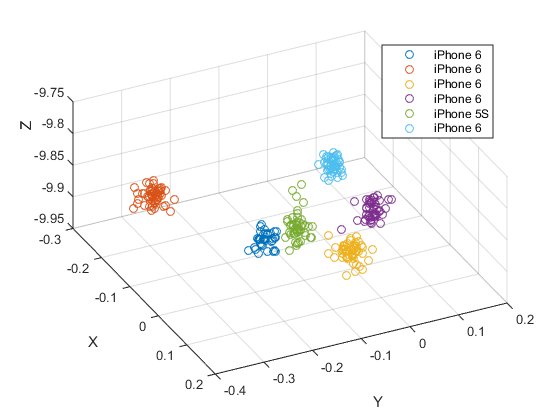
\includegraphics[scale=.6]{img/scatteriPhone}
\caption{Scatter-plot on accelerometer recordings of 6 Apple devices}
\label{fig:iPhoneScatter}
\end{figure}

\section{Result of measurements I  - Motion}\label{res:testI}
The data were gathered as described in~\sectionref{sec:measurementI} from the web-page in \figureref{fig:gyrotion} by spreading the the page. This resulted in over a hundred recordings, which had diversity in platforms, brands and models. Since the web-page where spread mostly to company employees the amount of devices with the same model is high as seen in ~\figureref{fig:measure1-topDevices}.
The purpose of this measurement where to identify if there where differences in terms of bias characteristics between the JavaScript's \texttt{accelerationIncludingGravity} and \texttt{acceleration}. The result of the measurements can be showed by making scatter-plots of the output acceleration of the devices. As shown in the ~\figureref{fig:measure1-topDevices} the \textit{Sony Xperia} devices represents more than a fifth of the total devices in the measurement. 
\begin{figure}[H]
	\centering
	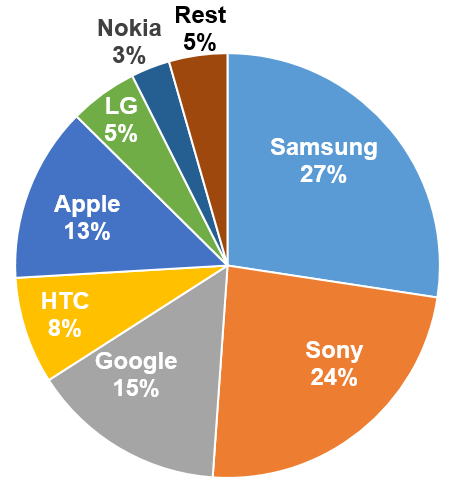
\includegraphics[scale=0.3]{img/measure1-brand}
	\caption{Diversity of device brand sampled in measurements I}
	\label{fig:measure1-brand}
\end{figure}
\begin{figure}[H]
	\centering
	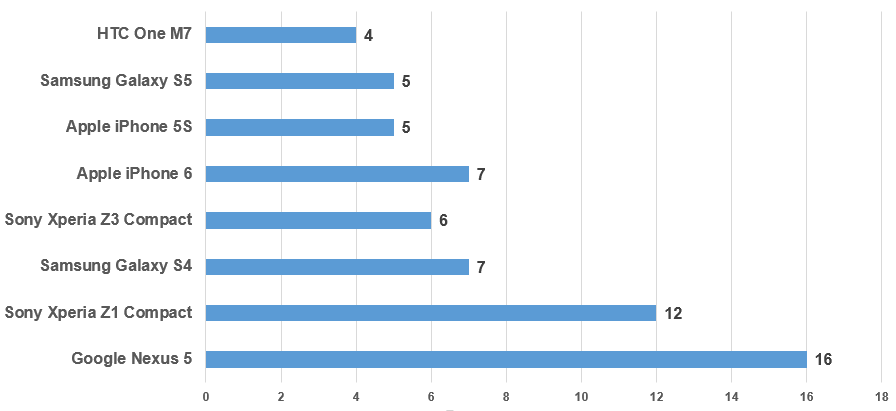
\includegraphics[scale=0.5]{img/measure1-devices}
	\caption{Most common devices models in measurements I}
	\label{fig:measure1-topDevices}
\end{figure}
The result of scatter-plots of measurements of 12 \textit{Sony Xperia} devices with and without gravity in accelerometer readings is shown in~\figureref{fig:scatter-withoutGrav} and~\figureref{fig:scatter-withGrav}.
\begin{figure}[H]
	\centering
	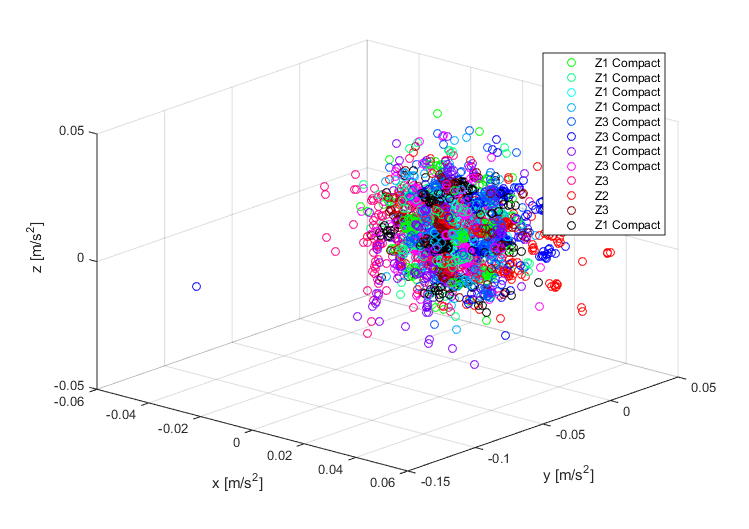
\includegraphics[scale=0.6]{img/res-measure1-scatter-notG}
	\caption{Bias from twelve \textit{Sony Xperia} deives measured with JavaScripts's \texttt{acceleration}}
	\label{fig:scatter-withoutGrav}
\end{figure}
\begin{figure}[H]
	\centering
	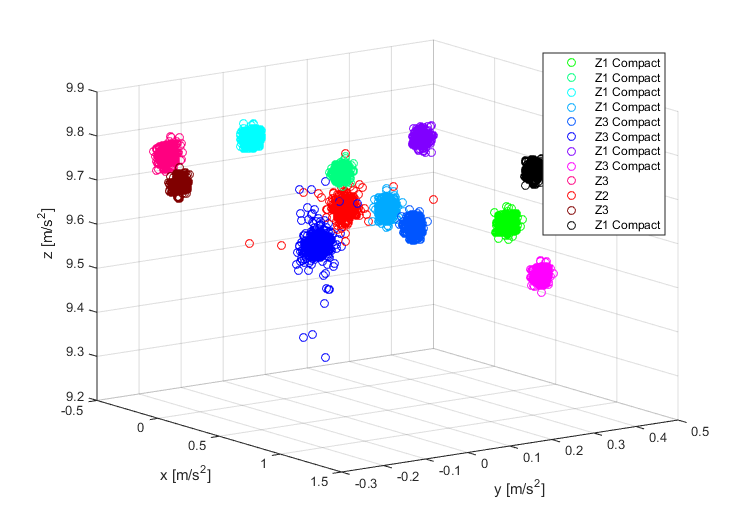
\includegraphics[scale=0.6]{img/res-measure1-scatter-inclG}
	\caption{Bias from twelve \textit{Sony Xperia} deives measured with JavaScripts's \texttt{accelerationIncludingGravity}}
	\label{fig:scatter-withGrav}
\end{figure}
As stated in~\cite{acc:kionixerr} the sources of bias in an accelerometer has to be compensated for. The manufacturer of the mobile devices makes some of this compensation before JavaScript gets the data. The results of the figures above indicates that JavaScript also makes compensating to the output of the event \texttt{acceleration}, probably to ease the development of software using the accelerometer, e.g. games. This however is not anything that is public in any specifications such~\cite{sensor:W3Cspec} or~\cite{sensor:accIncludingGravity}. The Android developer page about sensor event \cite{android:sensorEvent} state that they make factory calibration and temperature compensation even on their uncalibrated sensor events of (only magnetometer and gyroscope) that is relativity new feature added in Android 4.3 Jelly Bean (API level 18~\cite{android:API18}) from 2013 but the original once used since Android 1.5 Cupcake (API level 3~\cite{android:API3}) from 2009 makes some more noise compensation and calibration. What kind of compensation and calibration done is not public. 

\section{\textbf{Doing! }Result of measurements II  - Motion}\label{res:testII}
The result here is an analyses of the gyroscope and accelerometer data collected from 60 devices by an improved version of the JavaScript web-page used in measurements I. The changes that were made is described in~\sectionref{sec:measurementII} to improve that analyze data. \\
The diversity of the devices brands in the measurement is shown in the~\figureref{fig:brandII} below.
\begin{figure}[H]
	\centering
	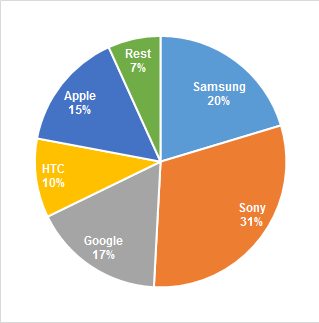
\includegraphics[scale=.4]{img/measure2-brands}
	\caption{Diversity of device brand sampled in measurements II}
	\label{fig:brandII}
\end{figure}

\subsection{Raw data result}
As in ~\cite{sensor:accelPrint} I used statistical features calculated by the time domain. The features used and calculated as followed:
\begin{figure}[H]
	\centering
	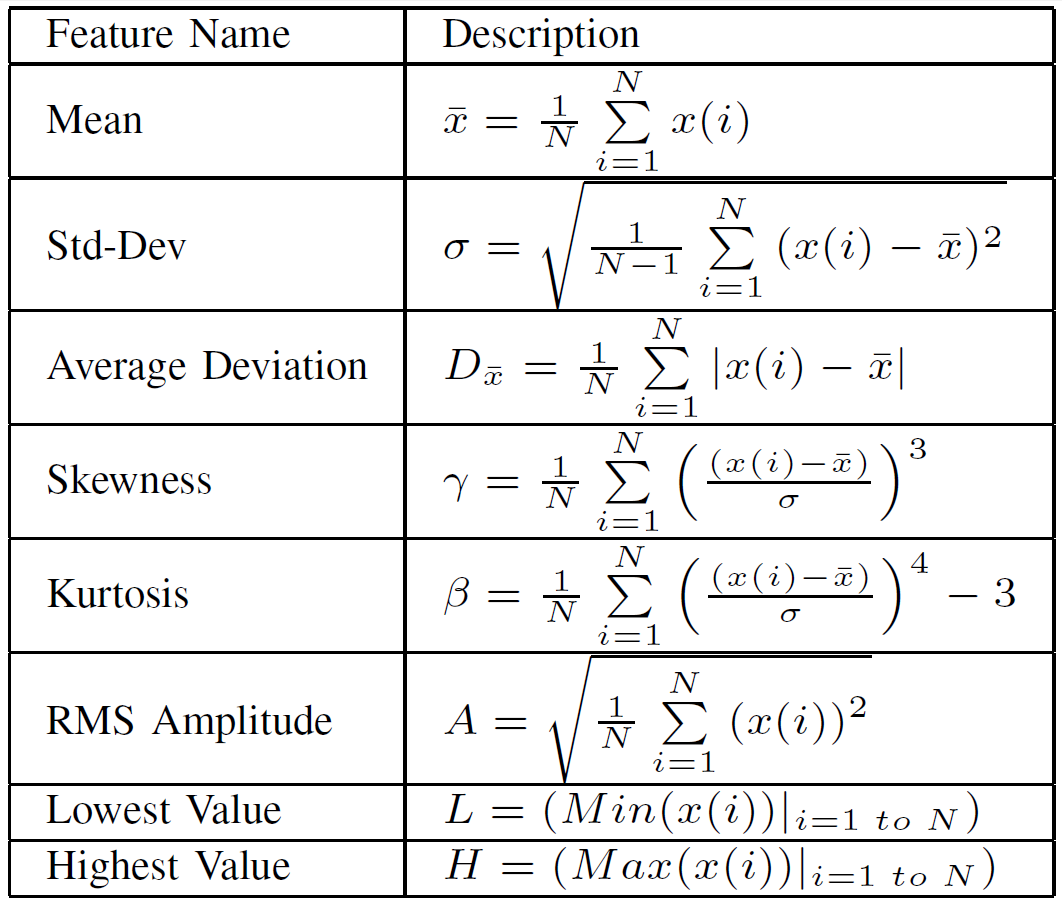
\includegraphics[scale=.35]{img/featureCalc}
	\caption{Calculations of statistical accelerometer features. \\\textit{From~\cite[p.6]{sensor:accelPrint}}}
	\label{fig:accFeatures}
\end{figure}

To know which features that separated the fingerprints of the devices the most the percentage of the distance between the features point were calculated as followed:
% \begin{enumerate}
% 	\item Extract vector $\overline{v}=\{\overline{x},\overline{y},\overline{z}\}}$ from each sample data of the devices .
% 	\item Calculated each feature for all $V_{n} = \{\overline{v_{1}},\overline{v_{2}},...,\overline{v_{n}}$
% 	\item Calculate the euclidean distance between all points for each feature in $V_{n}$ 
% 	\item Calculated the minimum and mean value of the euclidean distances
% 	\item The proportional differences between the distances $p=minimum/mean$, which gives the percentage of how close the minimum values are from each other. 	
% \end{enumerate}
This were formed in MATLAB on all of sampled data and the it resulted in the values of $p$:
\begin{table}[H]
	\centering
	\begin{tabular}{| p{4cm} | p{1cm} |}
	  Feature 			& $p$ 		\\ \hline
	  RMS Amplitude 	& 3.2\% 	\\
	  Skewness 			& 2.3\% 	\\
	  Average Deviation & 1.1\% 	\\
	  Highest value		& 0.36\% 	\\
	  Lowest value		& 0.50\% 	\\
	  Standard Deviation& 0.38\% 	\\
	  Mean 				& 0.31\% 	\\
	  Kurtosis 			& 0.30\% 	\\ \hline
	\end{tabular}
	\caption[Table caption text]{Comparing previous studies of camera fingerprinting} \label{table:prevCamera}
\end{table}
The order in the value above decides how the fingerprinting algorithm will decide if a device is matching or not. Since the values of 
\subsection{Accelerometer}

\subsubsection{Gyroscope}

\subsection{Permanence of accelerometer}
When choosing biometric trait one of the factors is permanence described in \sectionref{auth:bio:character}, that is the trait not changing significantly over time. To test this measurement II were performed on a \textit{Sony Xperia Z1 Compact} over a period of 50 days. The choice of device was based on that \textit{Sony Xperia} devices is 30\% of the devices that data is collected from. The same test were also made on a \textit{Google Nexus 7} tablet. The graphs below shows the difference of accelerometer readings over time.
\begin{figure}[H]
	\centering
	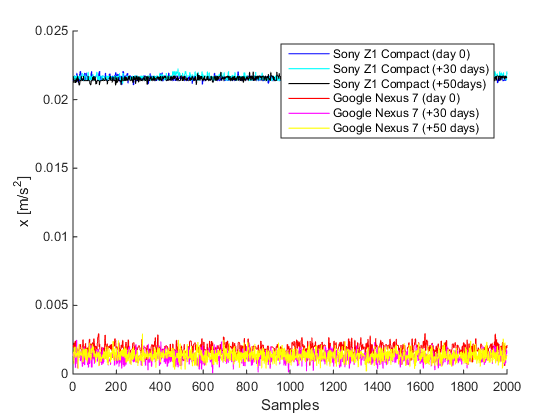
\includegraphics[scale=.7]{img/sensrec-nex-z1-acc-x}
	\caption{Accelerometer readings of x-axes on a  \textit{Sony Xperia Z1 Compact} and a \textit{Google Nexus 7} over 50 days}
	\label{fig:x50days}
\end{figure}
\begin{figure}[H]
	\centering
	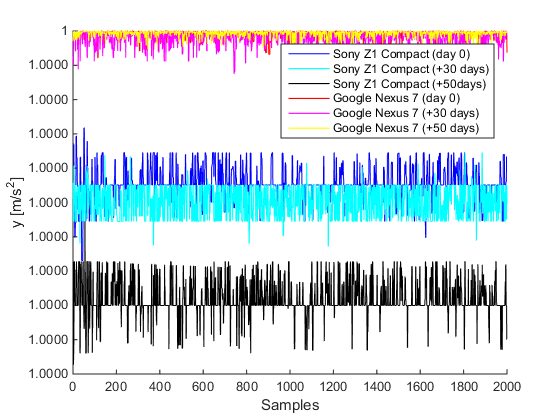
\includegraphics[scale=.7]{img/sensrec-nex-z1-acc-y}
	\caption{Accelerometer readings of y-axes on a  \textit{Sony Xperia Z1 Compact} and a \textit{Google Nexus 7} over 50 days}
	\label{fig:y50days}
\end{figure}
\begin{figure}[H]
	\centering
	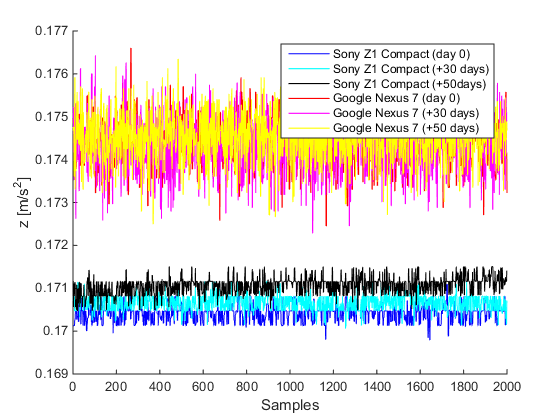
\includegraphics[scale=.7]{img/sensrec-nex-z1-acc-z}
	\caption{Accelerometer readings of z-axes on a  \textit{Sony Xperia Z1 Compact} and a \textit{Google Nexus 7} over 50 days}
	\label{fig:z50days}
\end{figure}
As seen in the figures the \textit{Google Nexus 7} hasn't changed much over the 50 days compared to the \textit{Sony Xperia Z1 Compact} that especially has changed in the y-axis. The reason for the difference of accelerometer change over time may be due to the \textit{Google Nexus 7} has only been in the same place during those 50 days and only used when the tests performed. Unlike Mobile used daily, may be dropped at some time. An additional fact about the measurements is that both devices has changed its OS between measurements 2 and 3. The \textit{Google Nexus 7} from Android KitKat 4.4.4 to Lollipop 5.1.1 and the \textit{Sony Xperia Z1 Compact} from Android KitKat 4.4.4 to CyanogenMod 12.1 ( Android version 5.1.1). \\
To get an perspective on this measurements among more devices the scatter-plot in~\figureref{fig:scatterSony50days} that include the same measurements from \textit{Sony Xperia Z1 Compact} as in~\figureref{fig:x50days},~\figureref{fig:y50days} and~\figureref{fig:z50days}.
\begin{figure}[H]
	\centering
	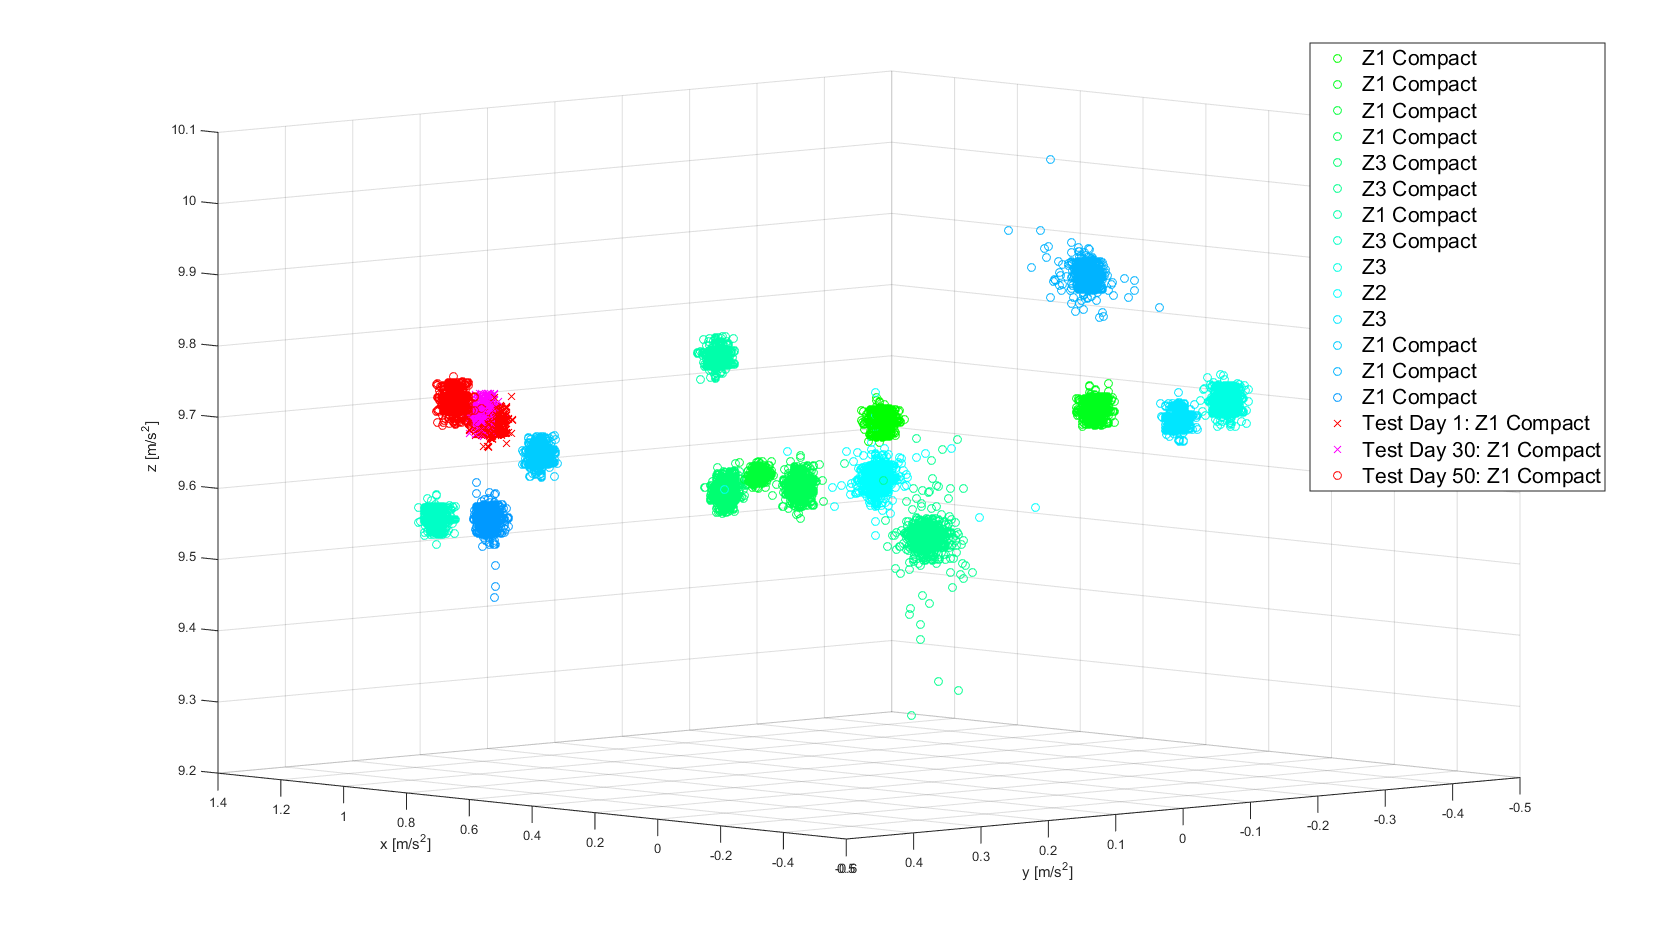
\includegraphics[scale=.3]{img/senrec-sony_scatter-2}
	\caption{Scatter-plot of accelerometer readings \textit{Sony Xperia}-device, one of them with measurements performed on the same device with 50 days apart.}
	\label{fig:scatterSony50days}
\end{figure}

\subsection{Simulate authentication of motion sensors in MATLAB}


% ========== CAMERA TEST ==========
\section{\textbf{ToUpdate! }Result Camera-measurements}\label{sec:ResCam}
\textbf{ ==== OBS!! ====}\\ Flyttad text som måste skrivas om.\\
\\
For the test of the camera sensor the PRNU value is calculated as an approximation of the algorithm described in section ~\ref{sec:char:camera} and also used by \cite{sensor:camera:DCIdent}. That is the average of multiple pictures used and substantially an approximation of \textit{f}. The first step is to remove the pictures-content which leaves the noise, which is done using a denoising filter. For the test the MATLAB \texttt{medfilt2} is used, which is an 2-D median filtering that outputs the median value of each pixel by its 3-by-3 neighbors. 
\begin{figure}[H]
  \centering
  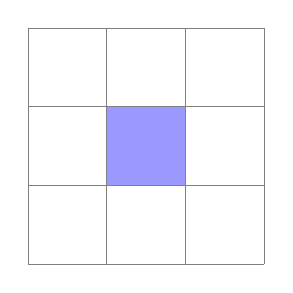
\begin{tikzpicture}[scale=1]
	\draw[step=1cm,gray,very thin] (0,0) grid (3,3);
	\fill[blue!40!white] (1,1) rectangle (2,2);
\end{tikzpicture}
  \caption{\label{fig:medfilt2} the MATLAB \texttt{medfilt2} outputs the median of each pixel by it's 3-by-3 neighbors}
\end{figure}
From the \texttt{medfilt2} we gain a picture without noise which is then subtracted from the original to get the noise. This technique works best if there are no features on the pictures such auto-fix, black and white etc. The more images used for the average value the better noise is, thus the amount random noise is less and the fixed noise is more. \cite{sensor:camera:DCIdent} recommend a minimum of 50 images. This is then seen as the reference pattern used for correlating the noise from another pictures. This correlation is calculated like:
$$
corr(\boldsymbol{n},\boldsymbol{r}) = 
\frac{(\boldsymbol{n} - \bar{\boldsymbol{n}})(\boldsymbol{r} - \bar{\boldsymbol{r}})}
{\|\boldsymbol{n} - \bar{\boldsymbol{n}}\| \|\boldsymbol{r} - \bar{\boldsymbol{r}}\|}
$$
A threshold for acceptance on correlation is found by experimental on images taken with or without the camera. Then there is a balance between FAR and FRR. 
In section ~\ref{sec:measurement:camera} i described two test preformed on the camera sensor of mobile devices.
\subsection{\textbf{ToDo! }Result of camera measurement I}
Since the purpose of this thesis compared to earlier work REFERENSER!! has the purpose of authentication and not forensics, is convenience for the collecting and measurability a factor to take in account. That is why the fist experiment is asked the users to record a 5 seconds video-clip with the device camera facing down on a flat object, like a table. Instead of making the user take 50 pictures or more which takes a lot of more time. This also makes it easier to get better noise since the same scene is used every time. \\
The video is then shuttled into images (100-200 from a 5 seconds video depending on fps on recording camera) that is used for calculating the PRNU. The MATLAB code for this is:\\
\rule{\textwidth}{0.5pt}
  \lstinputlisting{code/video2prnu1.m}
\rule{\textwidth}{0.5pt}

To compare an pictures between all collected PRNU the same calculation to get the noise is done. Then the noise from the reference pictures is compared to all collected PRNU and correlation is calculated like the formula above in MATLAB:\\
\rule{\textwidth}{0.5pt}
  \lstinputlisting{code/corrCamTest1.m}
\rule{\textwidth}{0.5pt}

\subsection{\textbf{ToDo! }Result of camera measurement II}
Since the earlier test leaved out some of the PRNU noise when recorded a video instead of taking a picture the new test consist of 10 images from every device. The recommendation from \cite{sensor:camera:DCIdent} to use at least 50 images is here compensated by again using black images (picture taking with device camera facing down). Since the scene is always the same the noise removal will be better in fewer images. The same code is used as above with the different that the video to image step is removed. The sizes of the images in this case is better since the camera on the mobile devices by default uses higher resolution when taking a picture then when recording. 

